\documentclass[a4paper, twoside, 11pt]{book}

% ============
% = PACKAGES =
% ============
\usepackage[utf8]{inputenc}
\def\labelitemi{--} % dash in itemize
\usepackage{booktabs} % in table, use of toprule, midrule and bottomrule
\usepackage{rotating} % allow to rotate a table
\usepackage[Lenny]{fncychap} % chapter customized typo
\usepackage[vscale=0.75,
            hscale=0.75, 
            hmarginratio=5:4, 
            vmarginratio=1:1, 
            marginparsep=5pt, 
            marginparwidth=2cm, 
            headheight=15pt]{geometry} % layout
\usepackage{graphicx} % graphics
\usepackage{amsmath, amssymb} % math
\usepackage{algorithm, algorithmic} %algorithms
\usepackage[tight]{subfigure} % subfigures
\usepackage{xspace} % space at end of macros
\usepackage{fancyhdr} % head of chapters (using lhead)
\usepackage{tabularx, caption}
\usepackage[square, sort&compress, numbers]{natbib}
\usepackage{pdfpages} % to insert a pdf right into the thesis
\usepackage[pagebackref=true, final, colorlinks=true]{hyperref} % hyperlinks
\usepackage{todonotes}
\newcommand{\chabstract}[1]{
\begin{quote}
\textbf{Abstract} {\footnotesize #1}
\end{quote}} % for chapter abstracts
\newcommand{\chconclu}[1]{
\begin{quote}
\textbf{Conclusion} {\footnotesize #1}
\end{quote}} % for chapter conclusions
\usepackage{minitoc} % mini content at the begining of each chapter
\usepackage{mathtools} % dcases environment: displaystyle automatically


\hypersetup{colorlinks=false} % for reading and printing

\graphicspath{{./FIGS/}{./PRIMITIVES/}{./CHAPTERS/HB/FIGS/}} % Specifies the directory where pictures are stored

% ================
% = NEW COMMANDS =
% ================
\newcommand{\ra}[1]{\renewcommand{\arraystretch}{#1}}

\begin{document}
\dominitoc % initialization of minitoc
\listoftodos
\cleardoublepage

% %!TEX root = ../../adrien_gomar_phd.tex

\chapter*{Abstract}
\thispagestyle{empty}

TEMP

\chapter*{Résumé}
\thispagestyle{empty}

TEMP


\tableofcontents
% \listoffigures

% \input{./CHAPTERS/nomenclature}

\mainmatter

% %!TEX root = ../main.tex

fil rouge:

"there is always a need for developing efficent methods for applications 
to blade designs. In a design cycle, a large number of flow solutions
are sought to interact iterativeley or concurrently with various options
opportunities and constraints from other disciplines"

% %!TEX root = ../main.tex

\chapter{Flow around contra-rotating open rotors: general information} % (fold)
\label{cha:cror}

\section{Introduction} % (fold)
\label{sec:introduction}
augmentation rendement moteur 
=> augmentation Overall Pressure Ration (par température d'entrée turbine 
ou mise en cascade de compresseurs)
ou augmentation du ByPass Ratio
CROR + AEL is justified

% section introduction (end)

\section{What is aeroelasticity ?} % (fold)
\label{sec:what_is_aeroelasticity_}

Aeroelasticity relies on the interaction of three forces:
the aerodynamic forces $\mathcal{A}$,
inertial forces $\mathcal{I}$ and elastic forces $\mathcal{E}$.
as depicted in Fig.~\ref{fig:COLLAR_TRIANGLE}.
\begin{figure}[htbp]
  \centering
  \includegraphics*[width=0.40\textwidth]{COLLAR_TRIANGLE.pdf}
  \caption{Collar's aeroelastic triangle}
  \label{fig:COLLAR_TRIANGLE}
\end{figure}
This diagram shows the relation between aerodynamic forces $\mathcal{A}$,
inertial forces $\mathcal{I}$ and elastic forces $\mathcal{E}$.
The forces are linked two by two to form: Static Aeroelasticity ($\mathcal{A} + \mathcal{E}$),
Structural Dynamics ($\mathcal{E} + \mathcal{I}$) and Flight Mechanics ($\mathcal{A} + \mathcal{I}$).
The interaction between these three forces can cause several issues such as:
\begin{itemize}
	\item divergence, which is a static aeroelastic phenomenon.
	It occurs when, for example, an airfoil has an axial stiffness that increases.
	Under aerodynamic loads, the trailing edge is stiffer than the leading
	edge, hence the fastest deflection of the leading edge which increases the
	angle of attack and thus the aerodynamic loads. This is a vicious circle that
	leads to the failure of the airfoil.
	\item flutter
	\item buffeting
	\item 
\end{itemize}

% section what_is_aeroelasticity_ (end)

\section{Aerodynamic of a Contra-Rotating Open Rotor} % (fold)
\label{sec:aerodynamic_of_a_contra_rotating_open_rotor}

In this section, we will detailed the different phenomena
arising in a Contra-Rotating Open Rotor.

\subsection{Introduction} % (fold)
\label{sub:introduction}

The Contra-Rotating Open Rotor denoted CROR in this thesis, sometimes
called Open Rotor or Unduct Fan, is an engine composed of 

% subsection introduction (end)

\subsection{Velocity triangle} % (fold)
\label{sub:velocity_triangle}

The CROR is designed to have no swirl at his outlet. In fact,
in a propeller, the main source of losses in terms
of efficiency comes from the swirl created downstream of
the rotor as mentioned above. This energy is wasted as the tangential component
of the velocity can not be used to generate thrust.
The basic idea behind the CROR technology is to put a
second contra rotating row that will transform this
tangential velocity to an axial velocity.
\begin{figure}[htbp]
  \centering
  \includegraphics*[width=0.40\textwidth]{VELOCITY_TRIANGLE_CROR}
  \caption{Velocity triangle for the CROR configuration.}
  \label{fig:VELOCITY_TRIANGLE_CROR}
\end{figure}

Figure~\ref{fig:VELOCITY_TRIANGLE_CROR} shows the velocity triangle for
a CROR configuration. Three vectors are depicted: the absolute velocity
$V$, the relative velocity $W$ and the rotation speed $U$. Between
the front rotor and the rear rotor, the rotation speed is inversed.
This





% subsection velocity_triangle (end)


% section aerodynamic_of_a_contra_rotating_open_rotor (end)

% chapter cror (end)

% 1. Flow around contra-rotating open rotors: general information
%     1.1 Background
%     1.2 Aerodynamic of an isolated propeller
%     1.3 Aerodynamic of a contra-rotating open rotor (avec review des simulations numériques déjà réalisées)
%     1.4 A few words on aeroelasticity
% - experimental aeroelasticity
% - numerical aeroelasticity: (contexte industriel aujourd’hui: plan de mélange pour du rotor/stator
% et on veut faire une matrice de calcul Mode / Dephasage => 360 pas possible)

%!TEX root = ../../adrien_gomar_phd.tex
\chapter{Spectral methods}
\label{cha:spectral_methods}

\chabstract{The spectral methods are presented in this chapter.
Actually four are presented: the Linearized 
Unsteady Reynolds-averaged Navier-Stokes (LUR), 
the NonLinear Harmonic (NLH), 
the NonLinear Frequency Domain (NLFD) 
and the Harmonic Balance (HB) method. The LUR
method comes from a linearization of the governing equation
while the three others are build to take into account for the 
non-linearities. The NLH, NLFD and HB methods
rely on the decomposition of the variable of interest
in Fourier series. By truncating these at order $N$,
$2N+1$ steady equations coupled by
a source term are developed. 
Emphasis is put on the development
of multi-frequential formulation and its
mathematical background to allow multi-stage
configurations.
The applicability of 
these methods is demonstrated in the literature
through analytical test cases, $2$D/$3$D academic 
turbomachine configurations,
industrial transonic multi-stage applications, 
aeroelastic configurations and even unsteady
optimization problems. The cost of the method
is almost $2N+1$ times the cost of a steady
computation with $N$ being the number of computed harmonics.}

% ================
% = INTRODUCTION =
% ================
\section{Introduction}
\label{sec:sm_intro}
%!TEX root = ../../../adrien_gomar_phd.tex

For an aircraft in steady flight conditions, 
lift balances weight and 
thrust balances drag. This explains why engineers try
indefinitely to reduce weight while increasing
thrust. A trade-off between those two is to work
on the propulsive efficiency of the engine. In this
section, general information on propulsion
that leads to the concepts of propeller and
contra-rotating open rotor are given.

\subsection{Thrust equation}
\label{sub:cror_thrust}
Consider the conservative equation of momentum
\begin{equation}
	\frac{\partial \rho \vec{V}}{\partial t} 
	+ \nabla \cdot (\rho \vec{V} \otimes \vec{V} + p \mathbb{I} - \vec{\vec{\Sigma}}_v) = 0,
\end{equation}
where $\rho$ is the density, $\vec{V}$ the velocity vector, $p$ the pressure and
$\vec{\vec{\Sigma}}_v$ the viscous stress terms.
Consider two closed domains $\Sigma$ and $\Sigma^\prime$ as
shown in Fig.~\ref{fig:cror_control_volume}.
\begin{figure}[htp]
  \centering
  \includegraphics*[width=0.30\textwidth]{control_volume.pdf}
  \caption{Domains used for the application of the momentum equation.}
  \label{fig:cror_control_volume}
\end{figure}
The domain $\Sigma^\prime$ represents a fluid domain outside from the
engine encompassed by the solid domain $\Sigma$.
Taking a steady state hypothesis, one can write
\begin{equation}
	\oint_{\Sigma} \left(\rho \vec{V} \otimes \vec{V} + 
	                       p \mathbb{I} - 
	                       \vec{\vec{\Sigma}}_v \right) \cdot \vec{n} \diff S
    =
   	\oint_{\Sigma^\prime} \left(\rho \vec{V} \otimes \vec{V} + 
	                       p \mathbb{I} - 
	                       \vec{\vec{\Sigma}}_v \right) \cdot \vec{n} \diff S,
\end{equation} 
where $\vec{n}$ is the normal vector.
As $\Sigma^\prime$ is an arbitrary domain, we can take it sufficiently
away from the engine so that $\vec{\vec{\Sigma}}_v$ becomes zero (\emph{i.e.}
viscosity stress terms are null).
Moreover, 
\begin{equation}
	\oint_{\Sigma} \left(\rho \vec{V} \otimes \vec{V} \right) \cdot \vec{n} \diff S = 0,
\end{equation}
since the surface is solid ($\vec{V} = \vec{0}$ on wall). 
If $\vec{F}$ denotes the resultant forces acting on $\Sigma$
\begin{equation}
	\vec{F} = \oint_{\Sigma} \left(p \mathbb{I} - 
	\vec{\vec{\Sigma}}_v \right) \cdot \vec{n} \diff S,
\end{equation}
then
\begin{equation}
	\vec{F} = \oint_{\Sigma^\prime} \left(\rho \vec{V} \otimes \vec{V} +
	p \mathbb{I} \right) \cdot \vec{n} \diff S.
\end{equation}
Assuming that $\Sigma^\prime$ is a stream tube, and projecting the equation
onto the $x$-axis gives the formula for the thrust $F_x$
\begin{equation}
	F_x = \dot{m} V_{out} + p_{out} S_{out}
	- \dot{m} V_{in} - p_{in} S_{in},
\end{equation}
using the notation of Fig.~\ref{fig:cror_control_volume}.

Far downstream of the engine $S_{in} = S_{out}$ and
considering that we have an adapted nozzle ($p_{in} = p_{out}$),
the thrust $F_x$ can be written as
\begin{equation}
	\fbox{$
	F_x = \dot{m} (V_{out} - V_{in}) = \dot{m} \Delta V_x
	$}
	\label{eq:cror_thrust}
\end{equation}
where $\dot{m}$ is the mass-flow rate going through the
propeller and $\Delta V_x$ is
the increment of axial velocity. From this simple equation,
one can see that to increase the thrust $F_x$, there are two parameters:
the mass-flow and the axial velocity increment.

\subsection{Global propulsive efficiency}
\label{sub:cror_efficiency}

The global propulsive efficiency $\eta$ measures the 
success in converting a mechanical power into a
propulsive power. It results from the combination
of the kinetic efficiency $\eta_{K}$ and the propulsive efficiency
$\eta_{PR}$
\begin{equation}
	\eta = \eta_{K} \times \eta_{PR}.
\end{equation}
This is schematically represented in Fig.~\ref{fig:cror_efficiency}.
\begin{figure}[htp]
  \centering
  \includegraphics*[width=0.40\textwidth]{efficiency.pdf}
  \caption{Efficiency relations from mechanical power to propulsive power.}
  \label{fig:cror_efficiency}
\end{figure}

\paragraph{Kinetic efficiency}
The kinetic efficiency measures the success in converting the mechanical
power $P_m$ into a kinetic power $P_k$
\begin{equation}
	\eta_K = \frac{P_k}{P_m}.
\end{equation}

The mechanical power delivered as input
can be computed through the first thermodynamic principle. In fact, in absence
of heat exchange, the mechanical power $P_m$ can be estimated as
\begin{equation}
	P_m = \dot{m} (h_{i_{out}} - h_{i_{in}}),
\end{equation}
where $h_i$ is the total enthalpy and subscript $in$ and $out$ are
the input and output, respectively, of the propulsion system as represented
in Fig.~\ref{fig:cror_control_volume}.
The kinetic power $P_k$ is given by
\begin{equation}
	P_k = \dot{m} \left(\frac{1}{2} V^2_{out} -
	\frac{1}{2} V^2_{in} \right).
\end{equation}
This leads to a kinetic efficiency that can be expressed as
\begin{equation}
	\eta_{K} = \frac{V^2_{out} - V^2_{in}}{2 (h_{i_{out}} - h_{i_{in}})}
\end{equation}

\paragraph{Propulsive efficiency}
The propulsive efficiency $\eta_{PR}$ measures the success
in creating a propulsive power $P_{pr}$ from a
kinetic power $P_k$
\begin{equation}
	\eta_{PR} = \frac{P_{pr}}{P_k}.
\end{equation}
The propulsive power is computed using the thrust $F_x$
\begin{equation}
	P_{pr} = F_x \times V_{\infty},
\end{equation}
where $V_{\infty}$ is the free-stream velocity.
Finally, if the free-stream velocity is the inlet velocity $V_{in}$
and the inlet and outlet velocities are purely axial
\begin{equation}
	\fbox{$
	\eta_{PR} = \displaystyle \frac{1}{1 + \frac{V_{out} - V_{in}}{2 V_{in}}}
	$}
	\label{eq:cror_propulsive_efficiency}
\end{equation}
This formula means that the most efficient engine produces
a very small velocity increment.

\subsection{Toward propeller engines}
\label{sub:cror_toward_propeller}

One way to improve the environmental footprint of
airplanes engines is to increase the propulsive efficiency
by reducing the kinetic power needed to drive the engine.
Doing so while maintaining the thrust can be achieved through
a higher mass-flow rate. Two new concepts are thus derived from
this simple statement: the High ByPass-Ratio (HBPR) which
is basically a turbofan with a larger fan exhaust, and the
propeller whose mass-flow rate is not limited
by the architecture, as the blades are not within a nacelle.
In the following section, the propeller engine will be detailed
and the drawbacks of such an architecture will be highlighted to
motivate the use
of a second propeller row, yielding the contra-rotating open rotor
architecture.




% ====================
% = STATE OF THE ART =
% ====================
\section{State of the art}
\label{sec:sm_state_of_the_art}
%!TEX root = ../../adrien_gomar_phd.tex

There is a large variety of spectral methods that exists in the
literature. The most important will be presented in this section.
As the development of these approaches on the Navier-Stokes equations
can be tedious, the following will only concentrate on the simplest
nonlinear equation, the advection equation for the velocity
defined as:
\begin{equation}
	\frac{\partial u}{\partial t} + 
	u \frac{\partial u}{\partial x} = 
	0.
	\label{eq:sm_nonlinear_convection}
\end{equation}
This equation can be formulated in a conservative manner for simplicity:
\begin{equation}
	\frac{\partial u}{\partial t} + 
	\frac{\partial}{\partial x} \left( \frac{u^2}{2} \right) = 
	0.
	\label{eq:sm_nonlinear_convection_conservative}
\end{equation}

The reader is referred to the cited papers for a detailed description
of the following methods and in particular, their
development for the Navier-Stokes equations. 

In total four spectral methods are presented, 
the Linearized Unsteady Reynolds averaged
Navier-Stokes, the NonLinear Harmonic method, the NonLinear Frequency Domain
method and the Harmonic Balance method.  
These names are chosen here
for simplicity but the reader might find in the literature many more
appellations. When it is the case, an effort will be made to synthesize
these to give the reader a good overview of the type of spectral methods available. 
Moreover, special emphasis will be put on the harmonic
balance method as it is the approach used in this thesis.


\subsection{The \underline{L}inearized 
\underline{U}nsteady \underline{R}eynolds-averaged Navier-Stokes method (LUR)}
\label{sub:sm_lur}
%!TEX root = ../../adrien_gomar_phd.tex

TO FILL

\subsection{The \underline{N}on\underline{L}inear 
\underline{H}armonic method (NLH)}
\label{sub:sm_nlh}
%!TEX root = ../../adrien_gomar_phd.tex

Originally developed by \citet{He1998} and \citet{Ning1998},
the NonLinear Harmonic method
relies on a decomposition of the conservative variables into a
time-averaged part plus an unsteady perturbation:
\begin{equation}
	u = \overline{u} + u^\prime,
	\label{eq:sm_nlh_decomposition}
\end{equation}
where $\overline{.}$ denotes the time-averaging operator and
$.^\prime$ the corresponding unsteady perturbation.
By injecting Eq.~\ref{eq:sm_nlh_decomposition} into
Eq.~\ref{eq:sm_nonlinear_convection_conservative}, one gets:
\begin{equation}
	\frac{\partial u^\prime}{\partial t} + 
	\frac{1}{2}\frac{\partial}{\partial x} \left[
	\overline{u}^2 + 2 \overline{u} u^\prime + u^\prime u^\prime \right] = 
	0.
	\label{eq:sm_nlh_step_1}
\end{equation}
The time-averaged equation can be obtained by time-averaging
equation~\ref{eq:sm_nlh_step_1}:
\begin{equation}
	(\overline{\ref{eq:sm_nlh_step_1}})
	\Leftrightarrow
	\frac{\partial}{\partial x}
	\left[\overline{u}^2 + 
	\overline{u^\prime u^\prime}\right] =
	0,
	\label{eq:sm_nlh_step_2}
\end{equation}
The term $\overline{u^\prime u^\prime}$
appears due to the non-linearities of the considered equation. It
is called the nonlinear stress terms 
(or the deterministic stress terms) as a reference to 
the Reynolds stress terms. 
The equations for the unsteady perturbations is then obtained by keeping
the first order terms of the unsteady equation~\ref{eq:sm_nlh_step_1}.
This means that the term $u^\prime u^\prime$ is neglected and leads
to:
\begin{equation}
	\frac{\partial u^\prime}{\partial t} + 
	\frac{\partial}{\partial x} \left[\overline{u} u^\prime \right] = 
	0.
\end{equation}

\paragraph{Mono-frequential formulation}
For now on, no assumption has been made neither on the velocity $u$,
nor on its time-averaged part and unsteady perturbation part.
Now, assuming that the velocity perturbation 
is periodic in time with period
$T=2 \pi / \omega$,
the unsteady fluctuations can be decomposed into 
a Fourier series:
\begin{equation}
	u^\prime = \sum_{k=-\infty \atop k \neq 0}^{\infty} 
	\widehat{u}_k e^{i \omega k t}.
	\label{eq:sm_nlh_decomposition_pert}
\end{equation}
Hence, since the complex exponentials forms 
an orthogonal basis, we have for all harmonics 
$-\infty \leq k \leq \infty, \; k \neq 0$:
\begin{equation}
	i \omega k \widehat{u}_k + 
	\frac{\partial}{\partial x} \left[ \overline{u} \widehat{u}_k\right] =
	0.
\end{equation}
One can notice that the time-averaged part has been removed from
the Fourier series through $k \neq 0$.
Each harmonic equation represents now a steady equation as no temporal
derivative is present anymore.

The term $\overline{u^\prime u^\prime}$ remains in the time-averaged
equation and needs to be computed. It can be 
directly worked out when the harmonics are known:
\begin{equation}
	\begin{split}
		u^\prime u^\prime &= 
		\left[
			\sum_{k=-\infty \atop k \neq 0}^{\infty} \widehat{u}_k e^{i \omega k t} 
		\right]
		\left[
			\sum_{k=-\infty \atop k \neq 0}^{\infty} \widehat{u}_k e^{i \omega k t} 
		\right] \\
		&= \sum_{k=-\infty \atop k \neq 0}^{\infty} (\widehat{u}_k)^2
		   e^{i 2 \omega k t} +
		   2 \sum_{j,k=-\infty \atop j \neq k \neq 0}^{\infty} 
		   \widehat{u}_k \widehat{u}_j e^{i \omega (j + k) t} \\
	\end{split}
\end{equation}
Thus,
\begin{equation}
	\begin{split}
		\overline{u^\prime u^\prime} &= 
		\frac{1}{T} \int_{t=0}^{T} \left[ 
			\sum_{k=-\infty \atop k \neq 0}^{\infty} (\widehat{u}_k)^2
		   	e^{i 2 \omega k t} +
		   	2 \sum_{j,k=-\infty \atop j \neq k \neq 0}^{\infty} 
		   	\widehat{u}_k \widehat{u}_j e^{i \omega (j + k) t} 
		\right] dt\\
		&= \frac{2}{T} \int_{t=0}^{T} \sum_{j,k=-\infty \atop j \neq k \neq 0}^{\infty} 
		   	\widehat{u}_k \widehat{u}_j 
		   	e^{i \omega (j + k) t} dt \\
		&= \frac{2}{T} \int_{t=0}^{T} 
			\sum_{k=-\infty \atop k \neq 0}^{\infty} 
			\widehat{u}_k \widehat{u}_{-k}  dt.
	\end{split}
\end{equation}
As $\widehat{u}_k$ and $\widehat{u}_{-k}$ are complex conjugates,
finally $\overline{u^\prime u^\prime}$ is equal to:
\begin{equation}
	\overline{u^\prime u^\prime} = 
	2 \sum_{k=-\infty \atop k \neq 0}^{\infty} |\widehat{u}_k|^2.
	\label{eq:sm_nlh_deterministic_stress_terms}
\end{equation}
This last equation depends only on the computed harmonics, meaning
that no term is modelled. Moreover, this term couples the
time-average solution with the unsteady perturbations. This is this
terms that is \todo{LUR}

Finally, as computing an infinite number of harmonics is not feasible,
the number of harmonics is truncated at order $N$. 
This is a fare assumption as most
of the physical flows have a finite unsteady spectrum. This
is for sure a reduce order approach. The goal of the spectral
methods being to have a compact representation of the unsteady time
signals. As for a mesh grid convergence, the number of harmonics $N$
is increased until the unsteady representation of the signal is
converged for the variable of interest. The discussion on the
convergence of spectral methods will be detailed later on in this 
thesis.

To summarize, the NonLinear Harmonic
method applied to Eq.~\ref{eq:sm_nonlinear_convection_conservative},
gives $2N + 1$ equations. A pseudo-time ($\tau$) derivative is
added to march the equations in pseudo-time to the steady-state 
solutions of all the harmonics:
\begin{equation}
	\fbox{$
	\begin{cases}
		\displaystyle \frac{\partial \overline{u}}{\partial \tau} + 
		\frac{\partial}{\partial x}
			\left[\overline{u}^2 + 
			\overline{u^\prime u^\prime}\right] &=
			0, \\
		\displaystyle \frac{\partial \widehat{u}_k}{\partial \tau} + 
		i \omega k \widehat{u}_k + 
			\frac{\partial}{\partial x} 
			\left[ \overline{u} \widehat{u}_k\right] &= 
			0, \: k \in [-N, N], \: k \neq 0,
	\end{cases}
	$}
	\label{eq:sm_nlh_subset_eq}
\end{equation}
coupled by the deterministic stress term $\overline{u^\prime u^\prime}$
defined in Eq.~\ref{eq:sm_nlh_deterministic_stress_terms}.
Three hypothesis lies under these equations:
\begin{itemize}
	\item the unsteady perturbations are periodic in time
	with period $T= 2 \pi / \omega$, 
	meaning that they can be decomposed into a Fourier series,
	\item the high-order cross-coupling terms $u^\prime u^\prime$
	are neglected,
	\item the number of harmonics is set to $N$.
\end{itemize}

\paragraph{Multi-frequential formulation}

In \citet{He2002}, the method is extended to a multi-frequential
perturbation. Instead of writing them
using a Fourier series as defined in Eq.~\ref{eq:sm_nlh_decomposition_pert},
these are written using a sum of harmonics each of which
having a frequency $\omega_k$:
\begin{equation}
	u^\prime = \sum_{k=-N \atop k \neq 0}^{N} 
	\widehat{u}_k e^{i \omega_k t}.
	\label{eq:sm_nlh_decomposition_pert_multi}
\end{equation}
Note that the term $k \omega$ in Eq.~\ref{eq:sm_nlh_decomposition_pert}
is now $\omega_k$ meaning that frequencies can be chosen
arbitrarily.
The derivation of the equations is kept the same and the following
$2N+1$ subset of equations are given:
\begin{equation}
	\fbox{$
	\begin{cases}
		\displaystyle
		\frac{\partial \overline{u}}{\partial \tau} +
		\frac{\partial}{\partial x}
			\left[\overline{u}^2 + 
			\overline{u^\prime u^\prime}\right] &=
			0, \\
		\displaystyle
		\frac{\partial \widehat{u}_k}{\partial \tau} + 
		i \omega_k \widehat{u}_k + 
			\frac{\partial}{\partial x} 
			\left[ \overline{u} \widehat{u}_k\right] &= 
			0, \: k \in [-N, N], \: k \neq 0.
	\end{cases}
	$}
	\label{eq:sm_nlh_subset_eq_multi}
\end{equation}
However, as the complex exponentials do not form
an orthogonal basis, writing Eq.~\ref{eq:sm_nlh_subset_eq_multi}
for each harmonic $k \in [-N, N], \: k \neq 0$ is mathematically
not true. In \citet{He2002}, they argue that the terms
are collected for each harmonic. 
The same development is made by \citet{Vilmin2006}.

The coupling deterministic stress term is evaluated using the
same equation as for the mono-frequential formulation.
In the multi-frequential formulation, 
the equation Eq.~\ref{eq:sm_nlh_deterministic_stress_terms}
is generally not true.
In fact, in the mono-frequential formulation, the term
\begin{equation}
	\frac{1}{T} \int_{t=0}^{T} (\widehat{u}_k)^2
		e^{i 2 \omega k t} dt
\end{equation}
vanishes for each $k$ as the integral of the
exponential $e^{i 2 \omega k t}$ with respect to $t$
is given by $e^{i 2 \omega k t} / 2 i \omega k$ that is
periodic with period $T$. However, in the multi-frequential
formulation, for some choice of frequencies, the period of all
of these may be difficult or even impossible to define. It
seems that mathematical justifications should be given
to be able to evaluate the deterministic stress term 
using Eq.~\ref{eq:sm_nlh_deterministic_stress_terms}.

\paragraph{Clocking effects}
In \citet{He2002}, the nonlinear harmonic method is extended to
compute all clocking position in one computation. Before
go into details of how this is done, let us explain what is
the clocking effect.
\begin{figure}[htbp]
  \centering 
    \subfigure{\includegraphics[width=.3\textwidth]{CLOCKING_EFFECT_1.pdf}}
    \subfigure{\includegraphics[width=.3\textwidth]{CLOCKING_EFFECT_2.pdf}}
    \subfigure{\includegraphics[width=.3\textwidth]{CLOCKING_EFFECT_3.pdf}}
  \caption{Different clocking positions for a stator/rotor/stator
  configuration.}
  \label{fig:sm_nlh_clocking_effect}
\end{figure}
Fig.~\ref{fig:sm_nlh_clocking_effect} displays three subfigures showing three
different clocking position in a stator/rotor/stator configuration.
As both stator are fixed, their relative position is of 
prior interest. The wake that is generated behind the first stator
is cut by the rotor blades but however almost convected up to 
the stator row. The stator being fixed, the wake generated
behind the first stator is seen stationary by the second stator.
Hence, the importance of their relative position. Here, the
first clocking position does not provide unsteadiness to the
last stator while the third clocking position gives the highest
level of unsteadiness in the stator. \todo{papier qui justifie
l'importance du calcul du clocking}

The brute force to compute the clocking effect on a
configuration is to consider all relative positions. This means
that the geometry of the stator should be rotated for each new 
clocking position. The innovative thinking proposed in 
\citet{He2002} is to consider the clocking effect as a steady wave.
In fact, as both stator are fixed, a steady perturbation
generated behind the first stator is still steady in the second stator.
In terms of frequencies, a steady perturbation is a perturbations 
whose frequency is zero. In \citet{He2002} and \cite{Vilmin2009}, 
a perturbation with a very small frequency (close to machine precision)
is computed. The clocking effect can then be evaluated by
post-processing the Fourier coefficient of the zero frequency mode.

Recently, the clocking effects \citet{Vilmin2013a}
\todo{à cmopléter}

\paragraph{Extension to the Navier-Stokes equations}

\paragraph{Applications}
The NonLinear Harmonic method 
has been succesfully implemented
in the NUMECA-Fine/Turbo solver by 
\citet{Vilmin2006, Vilmin2007, Vilmin2009, Vilmin2013a}.\todo{a améliorer + ajout frozen turbulence}

\subsection{The \underline{N}on\underline{L}inear 
\underline{F}requency \underline{D}omain method (NLFD)}
\label{sub:sm_nlfd}
%!TEX root = ../../adrien_gomar_phd.tex

\subsection{Mono-frequential formulation}

Originally proposed by \citet{McMullen2001}, the NLFD
method relies on a simple observation: to develop spectral methods, and in
particular the NLH method, one has made use of the Fourier
series to efficiently represent an unsteady signal.
This representation is then used to compute the unsteady
equation by converting it into $2N+1$ steady equations coupled by a 
source term where $N$ is small.
However, the method needs to be resolved in the frequency domain meaning
that all the numerical techniques should be adapted: the numerical schemes,
the turbulent models and so on. The smart idea 
proposed by \citet{McMullen2001} is to
make use of the fast Fourier Transform and its inverse to
allow it to be easily implemented into a classical time-domain code.
To explain the development of this method, let us first 
write Eq.~\eqref{eq:sm_nonlinear_convection_conservative} 
in a more general form:
\begin{equation}
	(\ref{eq:sm_nonlinear_convection_conservative})
	\Leftrightarrow
	\frac{\partial u}{\partial t} + R = 0,
	\label{eq:sm_nonlinear_convection_residual}
\end{equation}
with
\begin{equation}
	R = \frac{\partial}{\partial x} \left( 
	\frac{u^2}{2} \right).
\end{equation}
Let us now consider that both $u$ and $R$ are periodic
in time with respect to period $T = 2 \pi / \omega$
and can be written using a Fourier series:
\begin{equation}
	\begin{split}
		u(t) &= \sum_{k=-\infty}^{\infty} \widehat{u}_k e^{i k \omega t}, \\
		R(t) &= \sum_{k=-\infty}^{\infty} \widehat{R}_k e^{i k \omega t}.
	\end{split}
\end{equation}
Note that decomposing $R(t)$ into a Fourier series is equivalent
to use the Fourier decomposition of $u(t)$ and express
$R(t)$ using the Fourier coefficients $\widehat{u}_k$ of $u$
since the cross-terms that may arise are also expressed 
using the same complex exponentials. This comes from the fact
that multiplying a complex exponential with a complex exponential
just forms a new complex exponential at the power of the sum of the
two.
Injecting these decompositions into 
Eq.~\eqref{eq:sm_nonlinear_convection_residual} and taking into account
for the orthogonality of the complex exponentials:
\begin{equation}
	i k \omega \widehat{u}_k + \widehat{R}_k = 0, \: k \in [-\infty, \infty].
\end{equation}
As previously, only a small number of harmonics $N$ is kept and 
a pseudo-time ($\tau$) derivative is added to march the equations
in pseudo-time to the steady-state solutions of all the harmonics:
\begin{equation}
	\fbox{$
	\displaystyle \frac{\partial \widehat{u}_k}{\partial \tau} + 
	i k \omega \widehat{u}_k + \widehat{R}_k = 0, \: k \in [-N, N].
	$}
	\label{eq:sm_nlfd_subset_eq}
\end{equation}
The fact that $R(t)$ is expressed using its own Fourier series 
makes it simpler to implement 
as it avoid developing its expression using 
the complex coefficients $\widehat{u}_k$. 
However, $\widehat{R}_k$ must be evaluated. To do so, as depicted
in Fig.~\ref{fig:nlfd_principle}, \citet{McMullen2001}
propose to use an Inverse Fast-Fourier Transform (IFFT) to get
$u(t)$ from $\widehat{u}_k$. Then the considered governing equations
are used to evaluate $R(t)$ which leads to $\widehat{R}_k$
through a Fast-Fourier Transform (FFT). Finally, the next iteration value 
$\widehat{u}_k$
is evaluated by adding $\widehat{R}_k$ and 
the corresponding temporal derivative $i k \omega \widehat{u}_k$. All
harmonics are coupled through the IFFT and FFT operations
that needs all of the former to compute the counterpart temporal signal,
hence the coupling. Moreover, 
in the non-viscous Burger's equation framework, 
the term $u^\prime u^\prime$ is not neglected anymore compared to the
NLH approach and the computation of the deterministic stress is encompass
by the FFT and IFFT operations.
\begin{figure}[htbp]
  \centering
  \includegraphics*[width=0.50\textwidth]{nlfd_principle.pdf}
  \caption{Simplified diagram of the computation of $\widehat{R}_k$ from $\widehat{u}_k$
  for the non-linear frequency domain method.}
  \label{fig:nlfd_principle}
\end{figure}

\subsection{Extension to the Navier-Stokes equations}
The Navier-Stokes equations can be written in finite-volume,
semi-discrete form as:
\begin{equation}
	V \frac{\partial W}{\partial t} + R(W) = 0,
	\label{eq:navier_stokes_fv_sd}
\end{equation}
where $V$ is the volume of the cell and $W$
the vector of conservative variables.
This formulation is similar to
Eq.~\eqref{eq:sm_nonlinear_convection_residual} meaning that
nothing particular has to be made to derive this approach for
the Navier-Stokes equations. This is indeed attractive as the
method can be applied almost directly, except for the FFT and IFFT
step that should be added into the pseudo time loop.

\subsection{Time line}
\begin{figure}[htbp]
  \centering
  \includegraphics*[scale=0.6]{timeline_nlfd.pdf}
  \caption{Time line for the non-linear frequency domain method.}
  \label{fig:timeline_nlfd}
\end{figure}
Figure~\ref{fig:timeline_nlfd} shows the time line of the
development of the NLFD method.
The method was first introduced by \citet{McMullen2001}
and applied to the two-dimensional
Navier-Stokes equations. It has been validated against an
unsteady channel flow that admits an analytical 
solution~\cite{Merkle1987} and applied to a cylinder
vortex shedding. This could be done as the frequency of the
vortex shedding was known \emph{a priori} from experimental
and numerical data. However, for a given cylinder, it is not
possible to know this frequency. This is why
 \citet{McMullen2002, McMullen2006a}
proposed a gradient based method for determining the frequency
of a periodic phenomena where the frequency is unknown
\emph{a priori}. They argue that the frequency domain formulation
helps forming a gradient operator to find the period $T$ based
on the minimization of the residual of the unsteady equations.
They applied their algorithm to find the frequency of the vortex
shedding around a cylinder, and found it with a $3.5\%$ accuracy
compared to experimental data.
\citet{Nadarajah2003} compared an optimum shape design 
strategy for 
airfoils undergoing a change 
in angle of attack as a function of time 
using both a classical time-marching scheme
and the NLFD scheme within the Euler equations
framework. It is shown that the NLFD method
gives the same accuracy for the gradient and the optimum with only 
three time-instants ($N=1$)
compared to $23$ time-instants needed for 
the time-marching approach.
\citet{McMullen2006} evaluated all the acceleration techniques
that can be used with the NLFD method such as multigrid, local
time-stepping, residual averaging, coarse grid spectral viscosity,
proving that a steady-state convergence rate can be obtained.
Moreover, they compared the efficiency of the
NLFD method to a classical time-marching
scheme and showed that, for the same accuracy of the
solution, a one order to two orders of magnitude gain can
be obtained using the NLFD approach on a pitching airfoil.
\citet{Nadarajah2007} extended their optimum shape design strategy
using the NLFD to the three-dimensional Navier-Stokes equations.
A wing undergoing a change 
in angle of attack as a function of time is computed and
it is demonstrated that
five instants (namely two harmonics) is sufficient to provide
accurate results.
\citet{Kachra2008} extended the approach to the strong coupling of
aero-elasticity within the two-dimensional Euler equations framework.
They demonstrate that with a one-harmonic NLFD computation, the
flutter boundary of a NACA$64A010$ airfoil is correctly predicted.
This leads to a gain of one order of magnitude compared to a classical
time-marching procedure. Both the fluid dynamics and the structural equations
are solved using the NLFD approach. Moreover they quantitatively estimate the
cost of the FFT and IFFT done at each time-loop of the NLFD approach to be
approximately $2\%$ of the cost of one iteration, which is negligible.
\citet{Tatossian2011} extended the approach of \citet{Nadarajah2007}
to the aerodynamic shape optimization of hovering rotor blades
in the Euler framework.
First the NLFD approach is validated
against the Caradonna–Tung experimental blade.
The capability of 
their shape optimization process
to redesign this blade is assessed and gives a proof
of concept.
\citet{Mosahebi2013} implemented an adaptive NLFD approach named
the p-NLFD. Based on the energy of the last mode compared
to the whole spectrum, the number of harmonics
is increased if a fixed threshold is not reached.
A speed-up of $2$ in terms of CPU and
memory reduction is observed for the case of a
vortex-shedding behind a cylinder.




\subsection{Cost of the method}
The NLFD method is close to the NLH approach in terms of number
of equation solved. However, at each time-step a fast Fourier transform
is performed to cast back the harmonics into the time-domain in order
to compute the residual $R(t)$. \citet{McMullen2006} argue
that the cost of the fast Fourier transform is less than the cost of 
the spatial derivatives, and is thus negligible. This is 
confirmed by \citet{Kachra2008}.
Based on this affirmation, one can say that equivalent to the NLH
approach, if $\mathdollar_{\text{RANS}}$ 
denotes the CPU and memory cost of
one steady computation, the cost of the NLFD method can be 
approximated by:
\begin{equation}
	\mathdollar_{\text{NLFD}} = (2N+1) \cdot \mathdollar_{\text{RANS}}.
\end{equation}
This evaluation of the cost is confirmed by \citet{McMullen2002}.

% ====================
% = HARMONIC BALANCE =
% ====================
\section{The \underline{H}armonic \underline{B}alance method (HB)}
\label{sec:sm_hb}
%!TEX root = ../../adrien_gomar_phd.tex

The Harmonic Balance Technique proposed by \citet{Hall2002}
is a step further the non-linear frequency domain method. Instead
of using the fast Fourier transform to cast back the equations
to the time domain at each pseudo-iteration step, 
the equations are mathematically derived to 
computed into the time-domain.
To explain the method, we will use the general form of 
the viscous Burger's equation defined in 
Eq.~\ref{eq:sm_nonlinear_convection_residual}.

\subsection{Mono-frequential formulation}

Following the same approach as the non-linear frequency domain approach,
one consider that both $u$ and $R$ are periodic
in time with respect to period $T = 2 \pi / \omega$
and can be written using a Fourier series:
\begin{equation}
	\begin{split}
		u &= \sum_{k=-\infty}^{\infty} \widehat{u}_k e^{i k \omega t} \\
		R(t) &= \sum_{k=-\infty}^{\infty} \widehat{R}_k e^{i k \omega t}
		\label{eq:sm_hall_dft}
	\end{split}
\end{equation}
Injecting Eq.~\ref{eq:sm_hall_dft} in 
Eq.~\ref{eq:sm_nonlinear_convection_residual}, and considering
the orthogonality of the the complex exponentials:
\begin{equation}
	i k \omega \widehat{u}_k + \widehat{R}_k = 0, \: k \in [-N, N].
	\label{eq:sm_hall_frequential_eq}
\end{equation}

In the same way as one uses Fourier coefficients to
evaluate the temporal signal,
one can reconstruct the Fourier coefficients using
temporal evaluations taken at evenly spaced timelevels
sampling the period $T = 2 \pi / \omega$ using the forward
Fourier transform. Moreover, 
according to the Nyquist-Shannon~\cite{Shannon1949} sampling theorem, 
at least $2N+1$ timelevels are needed to capture $N$ frequencies,
leading to:
\begin{equation}
	\widehat{u}_k = \frac{1}{2N+1} 
	\sum_{n=0}^{2N} u_n^\star e^{-i k \omega t_n}.
\end{equation}
If $E$ denotes the matrix composed of the elements 
$E_{k,n} = e^{-i k \omega t_n} / 2N+1$, one can write $\widehat{u}_k$
and $\widehat{R}_k$ as:
\begin{equation}
	\begin{split}
		\widehat{u}_k &= E u^\star \\
		\widehat{R}_k &= E R^\star,
	\end{split}
	\label{eq:sm_matrix_fourier_operator}
\end{equation}
where $u^\star$ and $R^\star$ 
denote the vectors formed of all the evaluations of respectively $u$
and $R$,
made at $2N+1$ timelevels uniformly sampling the period of interest. 
$E$ can thus be named the inverse Fourier operator.
Note that conversely, using the Fourier operator $E^{-1}$:
\begin{equation}
	\begin{split}
		u^\star &= E^{-1} \widehat{u}_k \\
		R^\star &= E^{-1} \widehat{R}_k.
	\end{split}
\end{equation}

Injecting the matrix formulation of 
Eq.~\ref{eq:sm_matrix_fourier_operator} in 
Eq.~\ref{eq:sm_hall_frequential_eq}
gives:
\begin{equation}
	i K \omega E u^\star + E R^\star = 0,
\end{equation}
where $K$ is a diagonal matrix formed of all the $k \in [-N, N]$.
Now multiplying the equation by the Fourier operator $E^{-1}$:
\begin{equation}
	i \omega E^{-1} K E u^\star + R^\star = 0,
\end{equation}
where $R^\star$ can now be substituted:
\begin{equation}
	\fbox{$
		i \omega E^{-1} K E u^\star + 
		\displaystyle \frac{\partial}{\partial x}
		\frac{(u^\star)^2}{2} = 0
	$}
\end{equation}
What happened here is that instead of developing $R(t)$
in the frequency domain, which is tedious, this term is kept
as it is through all the development process. 
Since $R(t)$ only includes spatial derivatives, no non-linear
terms
rise from the Fourier decomposition. Hence, multiplying it
by the Fourier operator leads to the unity matrix. 
Finally $R(t)$ is simply evaluated at $2N+1$ timelevels.

This approach is really close to the non-linear frequency domain method.
The reader might observe that we are introducing the discrete Fourier
transform and its inverse. This is close to the fast Fourier transform
and it's inverse, as proposed by \citet{McMullen2001}. However,
as the development is on the equations and not during the time loop,
we get $2N+1$ steady equations that are coupled by a source term.
This source term appears as a spectral operator defined as:
\begin{equation}
	D_t = \frac{\partial E^{-1}}{\partial t} E = i \omega E^{-1} K E.
	\label{eq:sm_hb_mono_source_term_matrix}
\end{equation}
The main difference with the nonlinear frequency domain approach
is that the source term is known at the very first iteration and does
not change, meaning that we do not spend time computing a costly
fast fourier transform and its inverse at each time-step.

\citet{Gopinath2005} provide an analytical formulation of the
source term defined in Eq.~\ref{eq:sm_hb_mono_source_term_matrix}.
It a matrix operator whose elements are defined as:
\begin{equation}
  (D_t)_{l, j} =
  \begin{cases}
    \frac{\pi}{T}(-1)^{l-j}\csc\left(\frac{\pi
        (l-j)}{2N+1}\right) &, \, l\neq j,\\
    0 &, \, l=j.
  \end{cases}
\end{equation}


% ===================================
% = Periodic flows in turbomachines =
% ===================================
\section{Periodic flows in turbomachines}
\label{sec:sm_hudson}
%!TEX root = ../../adrien_gomar_phd.tex

As said in the introduction, the relative
velocity between two consecutive rows induces
unsteadinesses that can be correlated with the 
Blade Passing Frequency (BPF). A 

\chconclu{Four spectral methods have been presented in this chapter.
The main mathematical development have been demonstrated and 
the weakness/hypothesis of each method has been highlighted.
The large literature available on these methods shows that
they are ready for industrial, numerically hard
unsteady applications.}

% % 2. Spectral methods
% %     2.1 state of the art (Numeca / Duke / Stanford / Oxford /  Wyoming / Tenesse / ECL Thouverez)
% %     2.2 mono-frequential
% %         - theory
% %         - advantages
% %         - applications that can be treated
% %     2.3 multi-frequential (advantages and questions that it raises)
% %         - theory
% %         - advantages
% %         - applications that can be treated

% % 3. Advantages and limitations of spectral methods
% %!TEX root = ../main.tex
\chapter{Validation} % (fold)
\label{cha:validation}

\section{Presentation of the toy problems}

Two toy problems are set up to demonstrate
the capabilities and the limitations of the harmonic
balance approach, either mono-frequential or multi-frequential.




\section{Channel flow}
\label{sec:channel-flow}

\subsection{Test case description}
% presentation of the channel case
A channel configuration is set up to study the properties of the
proposed HB method and the above algorithms for non-uniform time
sampling.  It is a 2D channel of length $L_x = 100$~m in the axial
direction and $L_z = 1$~m in the transverse one.  The boundary
conditions are: (i)~an injection condition for the inlet,
(ii)~symmetric conditions for the upper and lower bounds as the flow
is assumed to be symmetric in the transverse direction, and (iii)~a
fluctuating pressure imposed at the outlet:
\begin{equation}
  P_{outlet}(t) = P_m \cdot \left[1 + A_1 \cdot \sin(2 \pi f_1 t) +
    A_2 \cdot \sin(2 \pi f_2 t) \right],
  \label{eq:outlet_canal}
\end{equation}
where $P_m$ is the temporal average static pressure, $A_n$ the
amplitude of the $n$\textsuperscript{th} mode and $f_n$ its
frequency. The mean outlet pressure $P_m$ is set to $60\%$ of the
inlet total pressure $P_{i0} = 101,325$~Pa.

Pressure waves travel within the flow with the velocity $u + c$ and $u
- c$, where $u$ denotes the local flow velocity and $c$ the sound
velocity. Since the pressure waves are generated at the outlet, only
the $u-c$ waves are visible, resulting in pressure waves propagating
upstream of the channel, which are damped by the effect of
viscosity. Figure~\ref{fig:canal_principle} shows a schematic diagram
of the channel case, illustrating the propagation and attenuation of
the pressure waves.
\begin{figure}[htb]
  \centering
  \includegraphics*[width=0.6\textwidth]{CANAL2_PRINCIPLE.eps}
  \caption{Schematic diagram of the channel case.}
  \label{fig:canal_principle}
\end{figure}

% mesh presentation
The mesh consists of 997~points along the axial direction and 9 in the
transverse one, which amounts to almost equal spacings in both
directions.


This configuration is turbulent as the Reynolds number based on the
inlet flow velocity and the axial length of the channel is about $R_e
\approx 2.0 \times 10^9$.  Turbulence is modeled using the
one-equation model of Spalart and Allmaras~\cite{Spalart1992}, and the
third-order upwind Roe scheme~\cite{Roe1981} is used to compute the
convective fluxes.

\subsection{Convergence sensibility analysis}

As mentioned previously, the condition number is of great importance
for the convergence of the proposed HB method. To highlight this
feature, the presented channel case is computed with a single
frequency at the outlet: $f_1 = 3$~Hz with an amplitude $A_1 = 0.05$
for the first case and $A_1=0.01$ for the second one, the second
frequency having a zero amplitude: $A_2= 0$.  Two frequencies are
specified for the HB computation: $f_1$ and its first harmonic
$2f_1$. The time levels are chosen to reach varying condition numbers
such that $1 \leq \kappa (A) \leq 3.43$.  Since the input frequencies of the HB
computation are harmonically related, the minimal conditioning
$\kappa(A) = 1$ is obtained with evenly spaced time levels.  The OPT
algorithm is modified by subtracting the targeted conditioning to the
objective function, so that the different condition numbers can be
reached.  The distribution of the time levels for each condition
number is shown in Fig.~\ref{fig:canal2_distribution_tlv}.  The time
levels deviate from the evenly spaced solution as the condition number
grows.
\begin{figure}[htb]
  \centering \subfigure[Relative to period
  $1/f_1$]{\includegraphics[width=.45\textwidth]{CANAL2_RESIDUAL_VS_CONDITIONNING_TLV_REPARTITION_F1.eps}}
  \quad \subfigure[Relative to period
  $1/2f_1$]{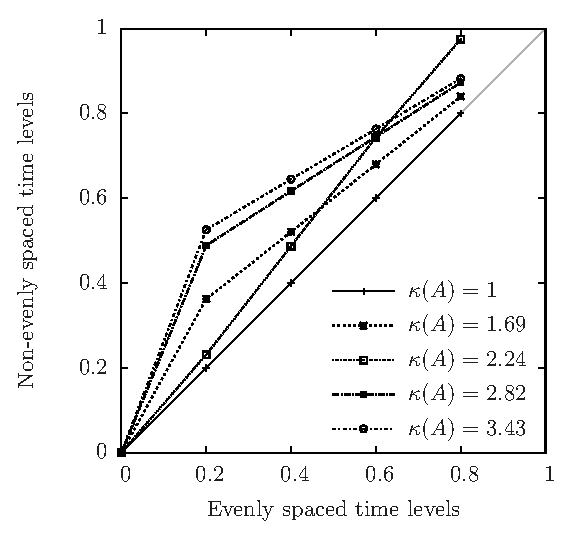
\includegraphics[width=.45\textwidth]{CANAL2_RESIDUAL_VS_CONDITIONNING_TLV_REPARTITION_F2.eps}}
  \caption{Distribution of the time levels on each frequency periods.}
  \label{fig:canal2_distribution_tlv}
\end{figure}
The results in Fig.~\ref{fig:canal_residual_vs_conditionning} show that
for a condition number $\kappa (A) \geq 3.43$ and wave input amplitude
$A_1 = 0.05$, the computation diverges. However, the computations with
the same condition numbers but a smaller input amplitude $A_1 = 0.01$
converge. In fact, the condition number amplifies the errors made
during the iterative process. When the input waves have a smaller
amplitude, the iterative errors are slighter, hence the convergence as
explained \S~\ref{sec:condition_number}.
\begin{figure}[htb]
  \centering \subfigure[$A_1 =
  0.01$]{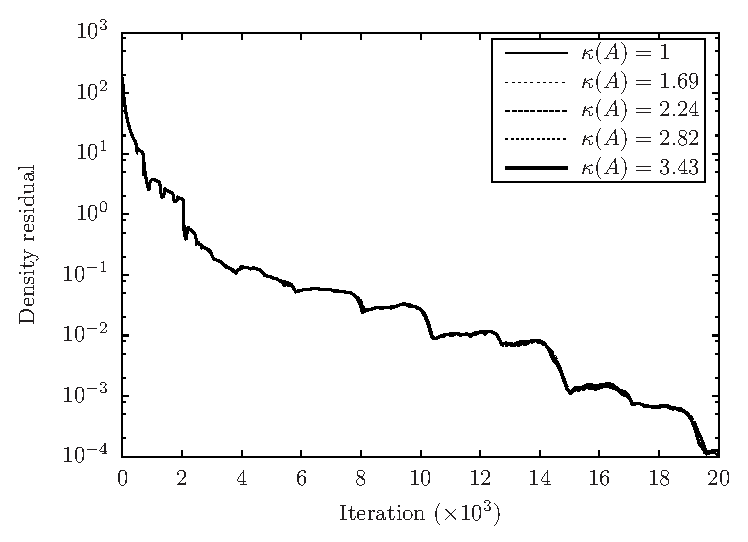
\includegraphics[width=.45\textwidth]{CANAL2_RESIDUAL_VS_CONDITIONNING_AMP001.eps}}
  \quad
  \subfigure[$A_1=0.05$]{\includegraphics[width=.45\textwidth]{CANAL2_RESIDUAL_VS_CONDITIONNING_AMP005.eps}}
  \caption{Relation between the condition number $\kappa (A)$ and the
    convergence of the solution.}
  \label{fig:canal_residual_vs_conditionning}
\end{figure}


\subsection{Validation of the multi-frequency HB method}

To validate the proposed HB method, two non-harmonically related
frequencies are chosen as input for the outlet boundary condition:
$f_1 = 3$~Hz and $f_2 = 17$~Hz.

A classical time-marching scheme is taken for comparison, namely the
Dual Time Stepping scheme (DTS~\cite{Jameson1991}).  The DTS method is
a 2\textsuperscript{nd}-order implicit time-marching scheme.
Convergence in time discretization is obtained after 20~periods using
160~instants per almost-period. Since the frequencies are integers and
coprime, the period is $T=1$~s.  Iterative convergence for the
inner loop is considered achieved when the normalized residuals drop
by $10^{-2}$ within a maximum of 50~sub-iterations.

The results obtained with the DTS scheme are compared to the HB
results for pressure waves amplitudes of $A = A_1 = A_2 = 0.001$.  The
transient of the DTS computation is shown
Fig.~\ref{fig:canal2_transient}, illustrating the wave propagation
with a slight attenuation of the high-frequency waves.
%The waves propagating upstream vanishing with the effect of viscosity
%are highlighted.
\begin{figure}[htbp]
  \centering
  \includegraphics*[width=.7\linewidth]{CANAL2_TRANSIENT.eps}
  \caption{DTS computation: transient propagation of the pressure waves.}
  \label{fig:canal2_transient}
\end{figure}


%Firstly, the DTS results are verified to yield a
%time-converged solution. =>deja dit plus haut !
The results are analyzed for frequencies $1<f< 40~\textrm{Hz}$ and the
dominant frequencies (the one that have the highest amplitudes) are
set for the HB computation.  To do so, pressure signals are probed
upstream, in the middle and downstream of the channel at
$x=[25~\textrm{m}, 50~\textrm{m}, 75~\textrm{m}]$ and $z=0.5$~m
respectively.  The spectrum of the aforementioned unsteady pressure
signals, obtained with a Fourier Transform, are plotted
Fig.~\ref{fig:canal2_dts_fft}.  The labeled frequencies are the
dominant ones, as for each probe, these have a high amplitude. They
are thus selected for the HB computation.  For such frequencies, the
OPT algorithm gives a set of time levels leading to a condition number
of~1.4.
\begin{figure}[htb]
  \centering
  \includegraphics*[width=.6\linewidth]{CANAL2_PROBE_POSITION.eps}

  \vspace{1em}

  \includegraphics*[width=.6\linewidth]{CANAL2_DTS_FFT.eps}
  \caption{Spectrum of pressure signals.}
  \label{fig:canal2_dts_fft}
\end{figure}

A Discrete Fourier Transform is computed at several axis positions,
resulting in the spatial evolution of the different harmonics, which
is used for the comparison of the HB and DTS approaches, in the middle
of the canal ($z = 0.5$~m).  In
Fig.~\ref{fig:canal2_validation_hbt_gear_amp_vs_axis}, the results are
plotted for the frequencies that have been set for the HB computation.
The overall agreement is fair.  Some local discrepancies can be
observed upstream for frequencies $f_2 + 3f_1$, $f_2 - f_1$ and $f_2 -
2f_1$. These are caused by aliasing
 but they are minimal regarding the temporal evolution, as
shown in Fig.~\ref{fig:canal2_validation_hbt_gear_time_ev}, where the
time evolution of pressure signals is extracted at all probes.  The
difference between the HB and the DTS method is negligible, proving
that the proposed HB method is able to reproduce the unsteady
almost-periodic phenomena.
\begin{figure}[htbp]
  \centering
  \includegraphics*[width=.7\linewidth]{CANAL2_VALIDATION_HBT_GEAR_AMP_VS_AXIS.eps}
  \caption{Spatial evolution of the amplitude of the dominant
    frequencies in the channel, for $f_1 = 3$~Hz and $f_2 = 17$~Hz.}
  \label{fig:canal2_validation_hbt_gear_amp_vs_axis}
\end{figure}

\begin{figure}[htb]
  \centering 
  \subfigure[Probe
  1]{\includegraphics[width=.45\textwidth]{CANAL2_VALIDATION_HBT_GEAR_TIME_EV_PROBE_1.eps}}
   \quad\subfigure[Probe
   2]{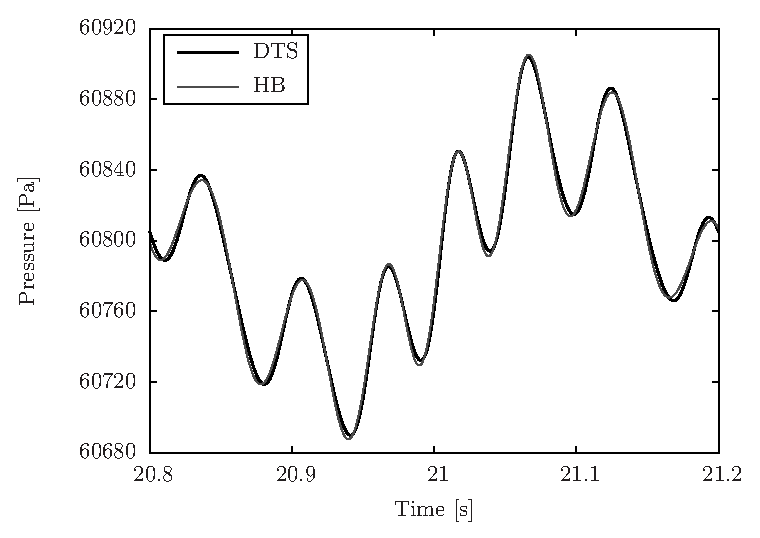
\includegraphics[width=.45\textwidth]{CANAL2_VALIDATION_HBT_GEAR_TIME_EV_PROBE_2.eps}}
   \subfigure[Probe
   3]{\includegraphics[width=.45\textwidth]{CANAL2_VALIDATION_HBT_GEAR_TIME_EV_PROBE_3.eps}}
  \caption{Unsteady pressure signals at different axial positions.}
  \label{fig:canal2_validation_hbt_gear_time_ev}
\end{figure}

The goal of this section was not to show significant CPU savings but
rather the capacity of the present HB method to capture an
almost-periodic flow on a model problem.  It is now applied to a more
complex configuration, namely a turbomachinery element, where its
computational efficiency is also emphasized.






\section{Convection equation solver}




% chapter validation (end)
% %     3.1 Presentation of the toy problem: convection equation
% %!TEX root = ../main.tex
\section{Advantages} % (fold)
\label{sec:advantages}

\subsection{Capturing a sinusoidal flow} % (fold)
\label{sub:capturing_a_sinusoidal_flow}

Harmonic balance approaches have been developed to
efficiently capture unsteady periodic signals.
In order to set these ideas on a simple example,
let us take the case of an injected signal composed
of the sum of two sine functions: 
\begin{equation}
	u_0(t) = \sin (2 \pi f_1 t) + \sin(2 \pi f_2 t).
\end{equation}




\subsubsection{case 1: $f_1 = f_2 = 1 \text{Hz}$}

This signal is made of a single frequency $f_1 = f_2 = 1 \text{Hz}$.
The mono-frequential harmonic balance computation ran with only one harmonic
is shown Fig.~\ref{fig:convection_sin_1_tsm_n_1}.
\begin{figure}[htbp]
  \begin{center}
    \includegraphics[width=.5\textwidth]{CONVECTION/FIGS/CONVECTION_SIN_1_TSM_N1.pdf}
  \end{center}
  \caption{Convection of a sinusoidal function. Harmonic balance computation
  ran with $f_1$ frequency compared to analytical result}
  \label{fig:convection_sin_1_tsm_n_1}
\end{figure}
The harmonic balance results match perfectly the analytical solution.
This was expected as harmonic balance methods have been developed to
easily capture periodic signals. When these are made of only one frequency,
one harmonic is sufficient to capture all the unsteadiness.

\subsubsection{$f_1 = 1 \text{Hz}$, $f_2 = 2 \text{Hz}$}

A sinusoidal function with a frequency $f_2 = 2f_1$ is now injected.
Two computations are ran. The first has 

\begin{figure}[htbp]
  \begin{center}
    \includegraphics[width=.5\textwidth]{CONVECTION/FIGS/CONVECTION_SIN_2_TSM_N1.pdf}
  \end{center}
  \caption{Convection of a sinusoidal function. Harmonic balance computation
  ran with frequency compared to analytical result}
  \label{fig:convection_sin_2_tsm_n_1}
\end{figure}

\begin{figure}[htbp]
  \begin{center}
    \includegraphics[width=.5\textwidth]{CONVECTION/FIGS/CONVECTION_SIN_2_TSM_N2.pdf}
  \end{center}
  \caption{Convection of a sinusoidal function.}
  \label{fig:convection_sin_2_tsm_n_2}
\end{figure}

\subsubsection{$f_1 = 1 \text{Hz}$, $f_2 = 10 \text{Hz}$}




\underline{What we have learned:} 
\begin{itemize}
  \item from case 1: For a sinusoidal temporal function made of only one frequency,
        only one frequency is needed to capture the field. This is much more efficient
        than a classical time-marching scheme.
\end{itemize}



% subsection capturing_a_sinusoidal_flow (end)

% section advantages (end)
% %     3.2 Advantages
% %         - capturing a periodic flow
% %     3.3 Limitations
% %         - condition of matrix A issue
% %             - highlighting the problem
% %             - solution: non evenly spaced timelevels & preconditionning ?
% \input{./CHAPTERS/algo_opt}
% %         - convergence
% %             - highlighting the problem
% %             - convergence of spectral methods: analyzing the spectrum of the wake
% %             - partial conclusion: we may go to industrial applications

% % 4. application to the aeroelasticity of contra-rotating open rotors
% %!TEX root = ../../main.tex
\chapter{Generalities}
\label{generalities}

\lhead{Chapitre ??. \emph{Generalities}}

\section{Equation solved} % (fold)
\label{sec:equation_solved}

The Unsteady Reynolds-Averaged Navier-Stokes (U-RANS) equations in
integral form are given by
\begin{equation}
   \int_\Omega \frac{\partial W}{\partial t} dV + \oint_{\partial
     \Omega} \overrightarrow{F} \cdot \overrightarrow{N} ds = 0,
   \label{eq:intNS}
\end{equation} 
where $\overrightarrow{F}$~is the flux across $\partial \Omega$ and
$W$~is the vector of the conservative unknowns (conservative variables
and turbulent variables).  Assuming $\Omega$ is a
control volume, the semi-discrete finite-volume form of the
U-RANS equations is obtained from Eq.~\eqref{eq:intNS}:
\begin{equation}
   \frac{d}{dt} \left(V  \overline{W}\right) + R \left( \overline{W}
   \right) = 0,
   \label{eq:semiDiscNS}
\end{equation} 
with $V$~the volume of the cell~$\Omega$, $R$~the residual resulting
from the discretization of the fluxes and the source terms (including
the turbulent equations), and $\overline{W}$ the mean of the
unknowns over the control volume.  In the following, the over line
symbol~$\overline{\cdot}$ is dropped out for clarity.

% section equation_solved (end)

% %     4.1 Presentation of elsA
% %         - schemes used
% %         - ALE/ aero-elasticity
% %!TEX root = ../../main.tex
\chapter{STCF 11}
\label{stcf11}

\lhead{Chapitre ??. \emph{Chapter Title Here}}

\section{Présentation de la configuration standard 11}
\label{sec:presentation_stcf11}

La configuration standard 11~\cite{Fransson:1999uq}
est une aube de stator de turbine oscillant sur 
son premier mode de flexion à régimes: un subsonique et un
transsonique. Le premier mode est 

\begin{table}[htbp]
  \ra{1.3} \centering
  \begin{tabular}{lccc}
    \toprule
    \phantom{abdefghijk}& $C_t$ & $C_p$ & $\eta$ \\
    \midrule
    Take-off & $-1.448$ & $2.895$ & $0.565$ \\
    Cruise & $-1.067$ & $5.32$ & $0.789$ \\
    \bottomrule
  \end{tabular}
  \caption{Point de fonctionnement.}
  \label{tab:flight_condition}
\end{table} 

\begin{itemize}
  \item un régime subsonique où l'écoulement
        ne présente pas de phénomènes physiques majeurs.
        Ce cas permet de facilement valider le code numérique
        avant de l'éprouver sur un point de fonctionnement plus
        complexe,
  \item un régime transsonique qui se distingue par la 
        présence d'un 
        choc à environ $75\%$ de la corde axiale,
        et d'un bulbe de décollement à $\approx 30\%$
        de la corde axiale.
        Ce cas permet, quant à lui, d'évaluer la robustesse
        du code dans le cas d'un écoulement complexe.
\end{itemize}

La cascade d'aubes est placée dans un canal annulaire fixe de l'École
Polytechnique Fédérale Lausanne~Fig.\ref{fig:canal_annulaire}.
Ce dernier permet d'obtenir un écoulement tant transsonique que subsonique
grâce à la forme de sa veine d'essai. De plus, le canal étant fixe,
l'instrumentation des pales est relativement aisée.
La vibration des pales est assurée par un actuateur électromagnétique
permettant la mise en place d'une onde tournante de type mode à diamètre.

\begin{figure}[htbp]
  \centering
  \includegraphics*[width=0.40\textwidth]{./ANNULAR_CHANNEL.pdf}
  \caption{Canal annulaire}
  \label{fig:canal_annulaire}
\end{figure}


\section{Instrumentation de l'aube}

L'instrumentation est réalisée sur la peau d'une des aubes.
Des sondes de pressions statiques non intrusives permettent
de mesurer la répartition de cette dernière 
le long de la corde axiale. Étant donné le caractère instationnaire
des phénomènes aéroélastiques, l'acquisition temporelle de la pression
statique est réalisée afin de donner les résultats sous forme de partie imaginaire
et réelle du premier harmonique de pression.

Pour la mise en valeur des effets stationnaires, le nombre de Mach isentropique est 
calculé à partir des mesures de pression statique. Ce dernier est défini par
% 
\begin{equation}
  M_{is} = \sqrt{\left[\left(\frac{P_{i0}}{P_s}\right)^{\frac{\gamma - 1}{\gamma}} - 1 \right] \cdot \frac{2}{\gamma -1}},
  \label{eq:mach_isentropique}
\end{equation}
% 
où $P_{i0}$ est la pression totale de référence et $P_s$ la pression statique
mesurée sur la peau de l'aube. Cette dernière évolue le long de la corde axiale.
Étant donné que $P_{i0}$ est constant, le nombre de Mach isentropique va suivre une
évolution similaire à l'inverse de la pression statique, ainsi il peut être
décrit comme l'interprétation de la pression statique sous forme de vitesse
adimensionnée, lorsque la pression totale n'est pas facilement accessible. En effet,
les aubes sont facilement instrumentées par des capteurs de pression statique, car ils 
ne nécessitent pas d'être intrusifs. Ceci est lié à la conservation de la
pression statique ($\frac{\partial P}{\partial n} = 0$ sous hypothèses de Prandtl). En revanche,
les prises de pression totale nécessitent de créer un arrêt isentropique, ce qui 
entraînerait la mise en place de sondes intrusives et de surcroît hors de la surface de
la peau de la pale.

Pour l'évaluation des effets aéroélastiques, des mesures de l'amplitude $\widetilde{Cp}$ et de la
phase $\widetilde{\phi}$ du premier harmonique de pression sont données sous forme de répartition
le long de la corde du profil définies par
% 
\begin{equation}
  \begin{split}
    C_{p, inst} &= \frac{c \cdot \widetilde{P_s}(x)}{h \cdot (P_{i0} - P_{s0})}, \\
    \widetilde{Cp} &= |C_{p, inst}|, \\
    \widetilde{\phi} &= \textrm{arg}(C_{p, inst}),
  \end{split}
  \label{eq:cp_inst}
\end{equation}
% 
où $\widetilde{P_s}(x)$ est l'évolution sur la corde du premier harmonique de pression
et $P_{s0}$ est la pression statique en entrée du canal.

La géométrie, les résultats expérimentaux et les articles associés à la 
configuration standard $11$ sont disponibles sur internet~\cite{STCF11_url}.
Des études sont présentes dans la littérature, principalement pour le cas 
transsonique de par la complexité de l'écoulement qui s'y développe 
\cite{Cinnella:2004fk, Sbardella:2001fk, Duta:2002uq, Campobasso:2003fk}.
Ces derniers montre l'adéquation des résultats numériques avec ceux expérimentaux, 
ce qui en fait un cas test intéressant.

\section{Paramètres numériques}

Le calcul est réalisé avec le code de calcul \textit{elsA}. Un schéma décentré de type
Roe du troisième ordre est choisi. Pour la modélisation de la turbulence, 
le modèle de Spalart-Allmaras est utilisé. Afin de pouvoir comparer les résultats obtenus
avec une approche de référence, les calculs instationnaires sont réalisés avec l'approche
classique dite de pas de temps dual.

L'aube de turbine est maillée en suivant une topologie O4H. Le nombre de points est de 160
autour de l'aube et les $y^+$ calculés sont $\mathcal{O}(1)$, ce qui correspond à l'état de 
l'art pour un tel calcul.

\section{Résultats stationnaires}

\subsection{cas subsonique}

Le cas subsonique est représentatif d'une turbine fonctionnant au point nominal.
L'écoulement ne présente pas de phénomènes particuliers~Fig.~\ref{fig:stcf11_rans_2D_subsonic}.
La répartition de nombre de Mach isentropique est 

\begin{figure}[htbp]
  \centering
  \includegraphics*[width=0.45\textwidth]{STCF11_SUBSONIC_FIELD_MIS_BW.png}
  \caption{Champ stationnaire}
  \label{fig:stcf11_rans_2D_subsonic}
\end{figure}

\begin{figure}[htbp]
  \centering
  \includegraphics*[width=0.45\textwidth]{STCF11_RANS_SUBSONIC.pdf}
  \caption{Répartition du nombre de Mach isentropique fonction de la corde axiale}
  \label{fig:stcf11_rans_mis_subsonic}
\end{figure}



\subsection{cas transsonique}

\begin{figure}[htbp]
  \centering
  \includegraphics*[width=0.45\textwidth]{STCF11_TRANSONIC_FIELD_MIS_BW.png}
  \caption{Champ stationnaire}
  \label{fig:stcf11_rans_2D_transonic}
\end{figure}

\section{Résultats instationaires}

\subsection{cas subsonique}

\subsection{cas transsonique}



% 
% Pour les simulations numériques, 
% 
% Les paramètres numériques utilisés pour les simulations suivantes sont rappelés ci-dessous:
% \begin{itemize}
%   \item schéma spatial de Roe d'ordre 3,
%   \item modèle de turbulence de type $k-l$ de Smith.
% \end{itemize}
% 
% \paragraph{Cartographie de champ 2D}
% 
% Les cartographies de champ 2D sont donnés en figure \ref{fig:stcf11_rans_2D}. La pression statique est représentée en contours et les lignes de courant en traits fins, ou en d'autres termes, la trajectoire que suit le fluide. Le cas subsonique ,\fig \ref{fig:stcf11_rans_2D_subsonic}, ne présente pas de singularité, le fluide accélère sur l'extrados et décélère sur l'intrados de la pale. En revanche, le cas transsonique présente de fortes singularités qui expliquent son étude à des fins de validation. En effet, ce dernier présente deux phénomènes aérodynamiques complexes repérés dans la figure \ref{fig:stcf11_rans_2D_transonic}. 
% \begin{itemize}
%   \item \textit{zone I}: bulle de décrochage. Avant que le profil décroche (c'est à dire que les lignes de courant ne suivent plus le profil), une bulle de décrochage peut se former. Or cette non-linéarité va réagir avec les vibrations de la pale comme nous le verrons plus tard.
%   \item \textit{zone II}: cette zone présente un choc. C'est un phénomène dimensionnant dans une turbomachine. On peut le visualiser par la discontinuité en pression qu'il présente.
% \end{itemize}
% 
% 
% \paragraph{Comparaison avec les résultats expérimentaux}
% Comme rappelé dans la section \ref{sec:presentation_stcf11}, des résultats stationnaires expérimentaux sont donnés sur le site internet du KTH. La comparaison avec les présents résultats est reportée en figure \ref{fig:stcf11_rans_expe}.
% 
% Ces résultats montrent la bonne adéquation entre l'expérience et les calculs numériques. Les principales disparités observées sont similaires à celle rencontrées dans la littérature:
% \begin{itemize}
%     \item cas subsonique: surestimation du Mach isentropique sur l'extrados de la configuration lors de la recompression,
%     \item cas transsonique: sous estimation de l'intensité du choc sur l'extrados et surestimation de la position du choc (zone II détaillé précédemment), même si les disparités dans les mesures expérimentales mettent en avant leurs incertitudes.
% \end{itemize}
% 
% 
% 
% \begin{figure}[H]
%     \center
%     \subfigure[cas subsonique]{ 
%       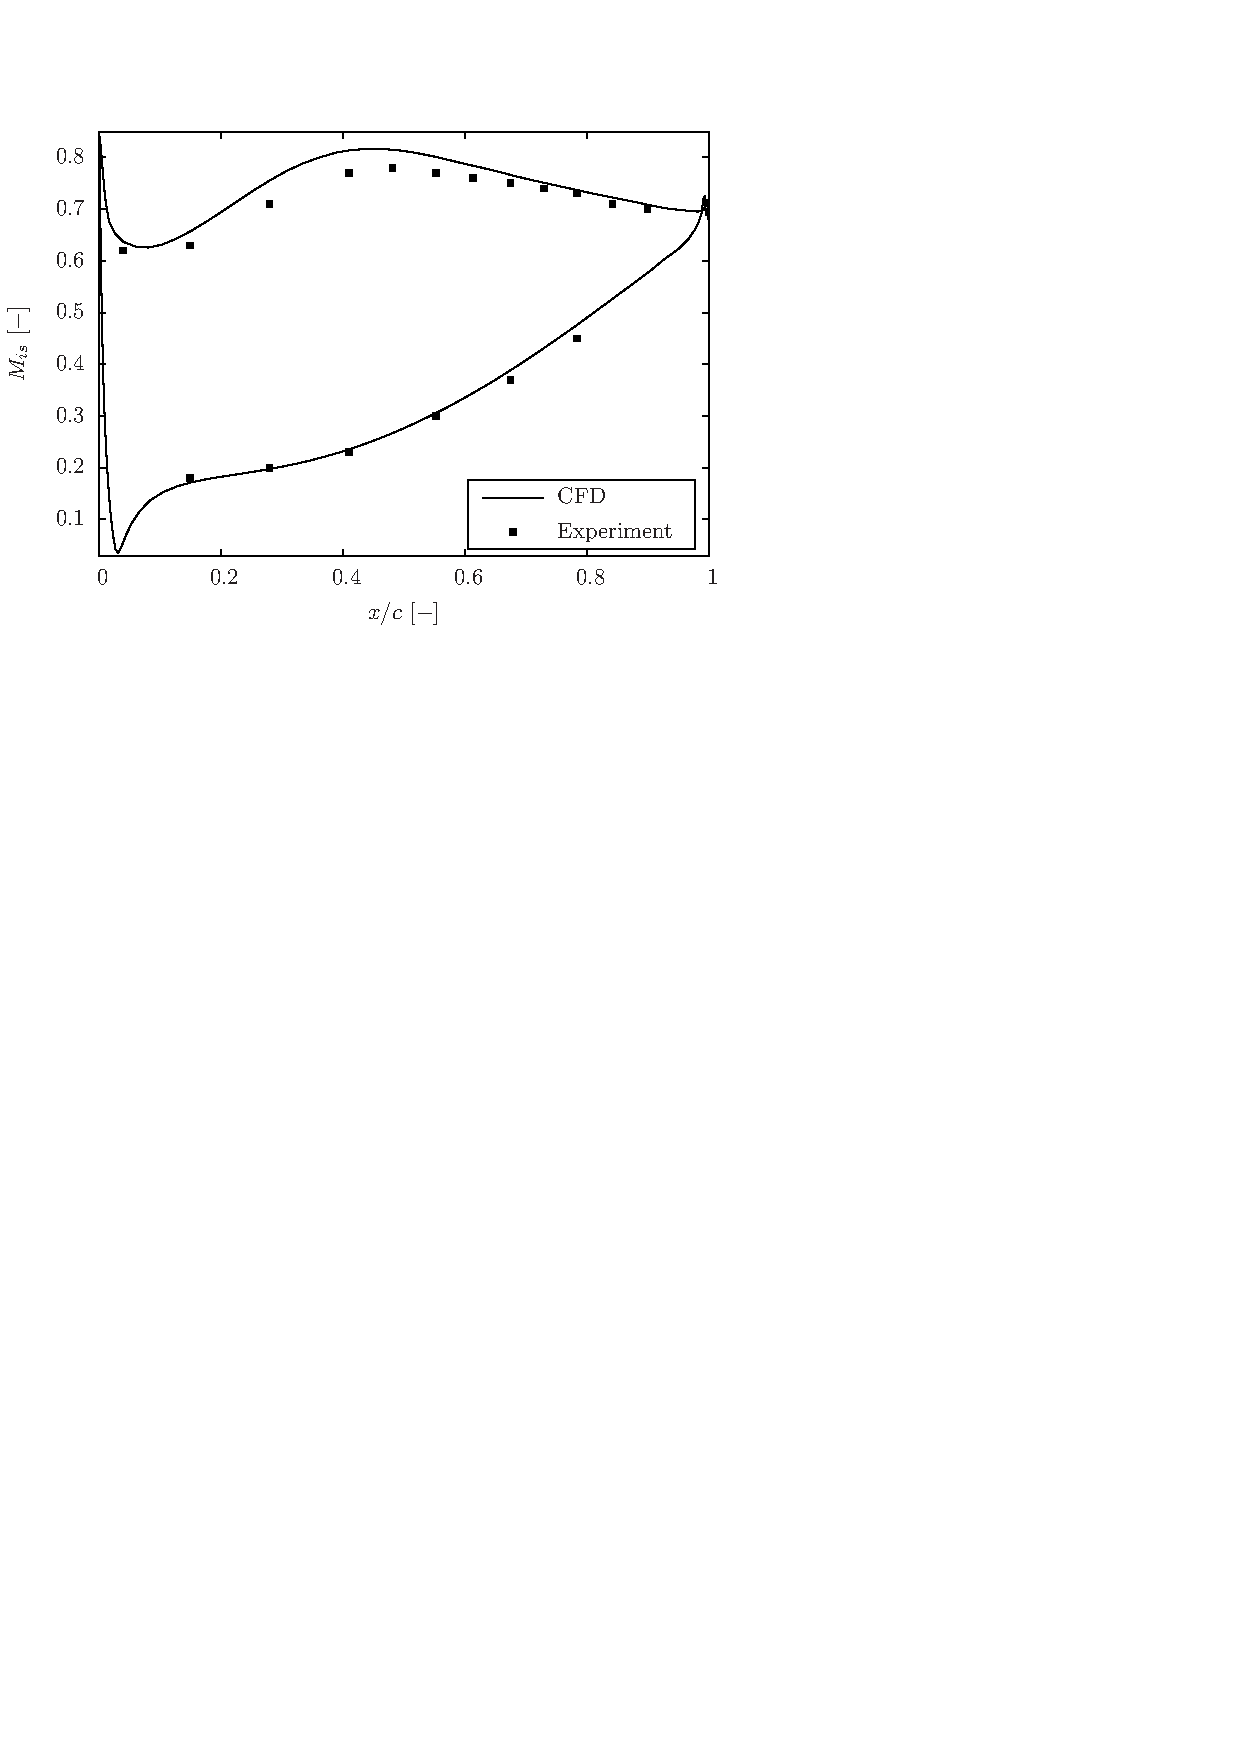
\includegraphics[width=7.5cm]{IMAGES/STCF11_RANS_SUBSONIC.pdf}}
%     \subfigure[cas transsonique]{ 
%       \includegraphics[width=7.5cm]{IMAGES/STCF11_RANS_TRANSONIC.pdf}}
%     \caption{Résultats stationnaires}
%     \label{fig:stcf11_rans_expe}
% \end{figure}
% 
% \section{Résultats aéroélastiques}
% 
% Des premiers résultats aéroélastiques ont été obtenus avec le code de calcul \elsa. La fréquence du mode imposé est $211.6 Hz$ et l'amplitude de $0.0035$.
% Les résultats sont donnés en terme d'évolution de l'amplitude et de la phase du premier harmonique de pression sur la pale. La figure \ref{fig:stcf11_ael} montre les résultats obtenus avec \elsa avec une approche DTS et HBT. Les résultats sont comparés à l'expérience et aux résultats de Cinnella et al. (voir Réf. \cite{Cinnella:2004fk}). En effet, les résultats numériques obtenus par ces derniers sont téléchargeables sur internet \footnote{http://cemec.poliba.it/BENCHMARK\_SC11.txt}, ce qui permet une comparaison supplémentaire.
% 
% L'analyse de ces résultats permet de dire que:
% \begin{itemize}
%   \item la prédiction des paramètres conditionnant l'amortissement est bonne que ce soit en DTS ou en HBT. Rien ne permet de qualifier l'une ou l'autre de meilleure. Ainsi, l'approche HBT pour prédire le flottement est validée,
%   \item les régions qui "pulsent" (comprendre où l'amplitude du coefficient de pression augmente) semble être les régions où il y a des phénomènes physiques importants. En effet, la région du bulbe de décrochage ($0 \leq x/c \leq 0.3$, zone I présentée dans la partie précédente) et la région du choc ($0.7 \leq x/c \leq 0.9$, zone II) ont toutes les deux un pic de coefficient de pression.
% \end{itemize}
% 
% 


% Fransson et al.:
% 
% - veine annulaire non tournante cascade de EPF-Lausanne
% - 20 pales excitée électromagnitiquement et contrôller pour vibrer en mode tournant
% - les suspensions des pales sont contruites afin de reproduire la fréquence propre
% et la direction du mode de flexion de la pale entrain de faire un movement rigide
% - STCF 11: choc droit à 75\% de la pale sur l'extrados
% - différences dans l'amortissement du à de petites différences dans la région du choc
% - mesures de pression totale et statique dans les plans e1 et e2 ainsi que derrière la cascade
% - les mesure pariétales sont faites au moyen de "pressure-taps" pour le cas stationnaires et de
% "miniaturized piezo-resistive pressure transducer" pour le cas instationnaire, embarqué à mi-hauteur de pale,
% sur différentes pales
% - en changeant un peu les conditions, le choc peut varier de 5\% en position
% - raisons de variations entre les expé et le numérique: effets du fluide réel non
% capté par les méthodes numérique ou perdu à cause des techniques de mesure (effet 3D, 
% couche limite des murs (hub/shroud), erreurs sur les relevés de pression, estimation des angles 
% du fluide, moyennage des grandeurs en azimuth et en hauteur radial)
% - amortissement varie énormement en fonction des conditions amonts
% dans le cas transsonique (fig 4.)
% - en revanche on a des tendances dans les mesures locales 
% - c'est la position du choc qui est la première source d'incertitude

% Cinnella et al.:
% 
% - pour les différents IBPA, elle multiplie le nb de canaux:
% np=z*360deg/IBPA, où z est l'entier minimum qui donne une valeur
% entière de np
% - présentation du cas STCF 11: conditions d'entrée (Mach et angle de l'écoulement)
% et reynolds de 1,2.10+6 basé sur la longueur de la corde et les conditions amonts
% - remise en cause de l'expé lorsque les bars de confiance à 95 \% sont de l'ordre
% de la valeur moyenne du point, gros écart lorsque Fransson et al. modifient les
% conditions amonts -> on regarde les résultats locaux

% Campobasso et Giles:
% 
% - ils font du LUR, couplage faible avec une méthode GMRES pour stabiliser
% les oscillations qu'ils obtiennent dans les champs stationnaires.
% - en fait ces oscillations sont dues à la physique du pb (décollement,
% vortex shedding ...)
% - ils imposent l'IBPA comme un déphasage complexe (comme nous)
% - ils calculent le travail du fluide sur la structure (donc pas les
% courbes d'amortissement de Fransson directement)

% Duta et al.:
% 
% - belle intro sur l'utilité de l'aéroélasticité
% - biblio sur méthodes de couplage faible
% - place du LUR dans simu aéroélastiques
% - LUR: hypothèse périodicité et petites perturbations
% - calcul adjoint pour estimer la réponse forcée de différents
% type de distortions amonts
% - si le sillage impacte la pale de manière uniforme, la réponse forcée sera maximale,
% si on a un déphasage du moment de l'impacte: déphasage=> minimisation
% du travail du fluide sur la structure

% Sbardella et Imregun
% 
% - papier de ref sur l'AEL
% - calculs 3D AEL bien mais les designers ont besoin de calculs qui tournent vite
% - le flottement est généralement un phénomène qui apparait dans des conditions off-design
% - sur prédiction sur le cas subsonique à mi-corde, mais raison de cet effet
% discuter dans Fransson et al.
% - nombre de Mach pré-choc est très sensible aux conditions d'entrée pour le 
% cas transsonique (fransson et al.), d'où les différences avec les essais
% - il vaut mieux que la turbulence ne soit pas gelée
% - rapport 30 sur le temps de calcul

% Fransson: Annular cascade experiments
% 
% - avantages de la veine d'essai annulaire non tournante:
%       * pas de murs latéral dans la direction circonférentielle => pas de réflexion des ondes de pression
%       * écoulement périodique dans le domaine
%       * instrumentation facile car pas de rotation
%       * écoulement supersonic possible grâce à la forme du tube d'écoulement
% - peut accueillir 20 pales
% - les pales sont en vibration forcée par le biais d'un exciteur électromagnétique
% la vibration des pales est mesurée par des capteurs de déplacement inductifs.
% ces capteurs sont fixés sur un anneau d'impact. Ce dernier est controllé axialement
% par un système hydraulique. Cela permet de limiter la vibration des pales si elles 
% commencent à osciller en flottement naturel (auto-déclanché) afin de ne pas casser
% les amortisseurs. Un système électronique de contrôle permet d'établir et de maintenir un 
% mode de vibration organisé de la cascade.
% - les frequences d'excitations doivent être proches de la fréquence propre 
% du système pale-mass-ressort
% %     4.2 validation of the proposed approach (STCF 11)
% %     4.3 aeroelasticity of an isolated contra-rotating open rotor
% %     4.4 Rotating block configuration: toward installed configurations
% %     4.5 [NOT SURE] aeroelasticity of an installed contra-rotating open rotor

%----------------------------------------------------------------------------------------
%	THESIS CONTENT - APPENDICES
%----------------------------------------------------------------------------------------

\addtocontents{toc}{\vspace{2em}} % Add a gap in the Contents, for aesthetics

\appendix % Cue to tell LaTeX that the following 'chapters' are Appendices

% Include the appendices of the thesis as separate files from the Appendices folder
% Uncomment the lines as you write the Appendices

% %!TEX root = ../main.tex
\chapter{Validation of the convection code}
\label{Appendix_convection_code}

%\input{./Appendices/AppendixB}
%\input{./Appendices/AppendixC}

\addtocontents{toc}{\vspace{2em}} % Add a gap in the Contents, for aesthetics

\backmatter

%----------------------------------------------------------------------------------------
%	BIBLIOGRAPHY
%----------------------------------------------------------------------------------------

\label{Bibliography}

\lhead{\emph{Bibliography}} % Change the page header to say "Bibliography"

\bibliographystyle{plainnat} % Use the "unsrtnat" BibTeX style for formatting the Bibliography

\bibliography{/Volumes/DATA/Users/gomar/Documents/Bibliographie/BibHBT/biblio_hbt,/Volumes/DATA/Users/gomar/Documents/Bibliographie/BibHBT/journal}

\end{document}  